\documentclass[1p]{elsarticle_modified}
%\bibliographystyle{elsarticle-num}

%\usepackage[colorlinks]{hyperref}
%\usepackage{abbrmath_seonhwa} %\Abb, \Ascr, \Acal ,\Abf, \Afrak
\usepackage{amsfonts}
\usepackage{amssymb}
\usepackage{amsmath}
\usepackage{amsthm}
\usepackage{scalefnt}
\usepackage{amsbsy}
\usepackage{kotex}
\usepackage{caption}
\usepackage{subfig}
\usepackage{color}
\usepackage{graphicx}
\usepackage{xcolor} %% white, black, red, green, blue, cyan, magenta, yellow
\usepackage{float}
\usepackage{setspace}
\usepackage{hyperref}

\usepackage{tikz}
\usetikzlibrary{arrows}

\usepackage{multirow}
\usepackage{array} % fixed length table
\usepackage{hhline}

%%%%%%%%%%%%%%%%%%%%%
\makeatletter
\renewcommand*\env@matrix[1][\arraystretch]{%
	\edef\arraystretch{#1}%
	\hskip -\arraycolsep
	\let\@ifnextchar\new@ifnextchar
	\array{*\c@MaxMatrixCols c}}
\makeatother %https://tex.stackexchange.com/questions/14071/how-can-i-increase-the-line-spacing-in-a-matrix
%%%%%%%%%%%%%%%

\usepackage[normalem]{ulem}

\newcommand{\msout}[1]{\ifmmode\text{\sout{\ensuremath{#1}}}\else\sout{#1}\fi}
%SOURCE: \msout is \stkout macro in https://tex.stackexchange.com/questions/20609/strikeout-in-math-mode

\newcommand{\cancel}[1]{
	\ifmmode
	{\color{red}\msout{#1}}
	\else
	{\color{red}\sout{#1}}
	\fi
}

\newcommand{\add}[1]{
	{\color{blue}\uwave{#1}}
}

\newcommand{\replace}[2]{
	\ifmmode
	{\color{red}\msout{#1}}{\color{blue}\uwave{#2}}
	\else
	{\color{red}\sout{#1}}{\color{blue}\uwave{#2}}
	\fi
}

\newcommand{\Sol}{\mathcal{S}} %segment
\newcommand{\D}{D} %diagram
\newcommand{\A}{\mathcal{A}} %arc


%%%%%%%%%%%%%%%%%%%%%%%%%%%%%5 test

\def\sl{\operatorname{\textup{SL}}(2,\Cbb)}
\def\psl{\operatorname{\textup{PSL}}(2,\Cbb)}
\def\quan{\mkern 1mu \triangleright \mkern 1mu}

\theoremstyle{definition}
\newtheorem{thm}{Theorem}[section]
\newtheorem{prop}[thm]{Proposition}
\newtheorem{lem}[thm]{Lemma}
\newtheorem{ques}[thm]{Question}
\newtheorem{cor}[thm]{Corollary}
\newtheorem{defn}[thm]{Definition}
\newtheorem{exam}[thm]{Example}
\newtheorem{rmk}[thm]{Remark}
\newtheorem{alg}[thm]{Algorithm}

\newcommand{\I}{\sqrt{-1}}
\begin{document}

%\begin{frontmatter}
%
%\title{Boundary parabolic representations of knots up to 8 crossings}
%
%%% Group authors per affiliation:
%\author{Yunhi Cho} 
%\address{Department of Mathematics, University of Seoul, Seoul, Korea}
%\ead{yhcho@uos.ac.kr}
%
%
%\author{Seonhwa Kim} %\fnref{s_kim}}
%\address{Center for Geometry and Physics, Institute for Basic Science, Pohang, 37673, Korea}
%\ead{ryeona17@ibs.re.kr}
%
%\author{Hyuk Kim}
%\address{Department of Mathematical Sciences, Seoul National University, Seoul 08826, Korea}
%\ead{hyukkim@snu.ac.kr}
%
%\author{Seokbeom Yoon}
%\address{Department of Mathematical Sciences, Seoul National University, Seoul, 08826,  Korea}
%\ead{sbyoon15@snu.ac.kr}
%
%\begin{abstract}
%We find all boundary parabolic representation of knots up to 8 crossings.
%
%\end{abstract}
%\begin{keyword}
%    \MSC[2010] 57M25 
%\end{keyword}
%
%\end{frontmatter}

%\linenumbers
%\tableofcontents
%
\newcommand\colored[1]{\textcolor{white}{\rule[-0.35ex]{0.8em}{1.4ex}}\kern-0.8em\color{red} #1}%
%\newcommand\colored[1]{\textcolor{white}{ #1}\kern-2.17ex	\textcolor{white}{ #1}\kern-1.81ex	\textcolor{white}{ #1}\kern-2.15ex\color{red}#1	}

{\Large $\underline{12a_{0898}~(K12a_{0898})}$}

\setlength{\tabcolsep}{10pt}
\renewcommand{\arraystretch}{1.6}
\vspace{1cm}\begin{tabular}{m{100pt}>{\centering\arraybackslash}m{274pt}}
\multirow{5}{120pt}{
	\centering
	\includegraphics[width=112pt]{../../../GIT/diagram.site/Diagrams/png/1699_12a_0898.png}\\
\ \ \ A knot diagram\footnotemark}&
\allowdisplaybreaks
\textbf{Linearized knot diagam} \\
\cline{2-2}
 &
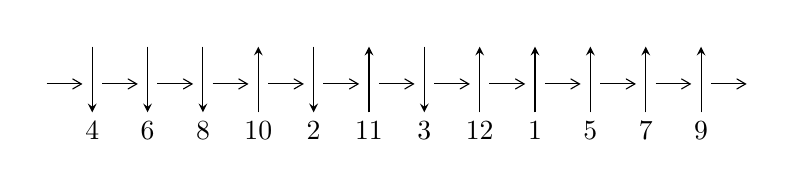
\begin{tikzpicture}[x=20pt, y=17pt]
	% nodes
	\node (C0) at (0, 0) {};
	\node (C1) at (1, 0) {};
	\node (C1U) at (1, +1) {};
	\node (C1D) at (1, -1) {4};

	\node (C2) at (2, 0) {};
	\node (C2U) at (2, +1) {};
	\node (C2D) at (2, -1) {6};

	\node (C3) at (3, 0) {};
	\node (C3U) at (3, +1) {};
	\node (C3D) at (3, -1) {8};

	\node (C4) at (4, 0) {};
	\node (C4U) at (4, +1) {};
	\node (C4D) at (4, -1) {10};

	\node (C5) at (5, 0) {};
	\node (C5U) at (5, +1) {};
	\node (C5D) at (5, -1) {2};

	\node (C6) at (6, 0) {};
	\node (C6U) at (6, +1) {};
	\node (C6D) at (6, -1) {11};

	\node (C7) at (7, 0) {};
	\node (C7U) at (7, +1) {};
	\node (C7D) at (7, -1) {3};

	\node (C8) at (8, 0) {};
	\node (C8U) at (8, +1) {};
	\node (C8D) at (8, -1) {12};

	\node (C9) at (9, 0) {};
	\node (C9U) at (9, +1) {};
	\node (C9D) at (9, -1) {1};

	\node (C10) at (10, 0) {};
	\node (C10U) at (10, +1) {};
	\node (C10D) at (10, -1) {5};

	\node (C11) at (11, 0) {};
	\node (C11U) at (11, +1) {};
	\node (C11D) at (11, -1) {7};

	\node (C12) at (12, 0) {};
	\node (C12U) at (12, +1) {};
	\node (C12D) at (12, -1) {9};
	\node (C13) at (13, 0) {};

	% arrows
	\draw[->,>={angle 60}]
	(C0) edge (C1) (C1) edge (C2) (C2) edge (C3) (C3) edge (C4) (C4) edge (C5) (C5) edge (C6) (C6) edge (C7) (C7) edge (C8) (C8) edge (C9) (C9) edge (C10) (C10) edge (C11) (C11) edge (C12) (C12) edge (C13) ;	\draw[->,>=stealth]
	(C1U) edge (C1D) (C2U) edge (C2D) (C3U) edge (C3D) (C4D) edge (C4U) (C5U) edge (C5D) (C6D) edge (C6U) (C7U) edge (C7D) (C8D) edge (C8U) (C9D) edge (C9U) (C10D) edge (C10U) (C11D) edge (C11U) (C12D) edge (C12U) ;
	\end{tikzpicture} \\
\hhline{~~} \\& 
\textbf{Solving Sequence} \\ \cline{2-2} 
 &
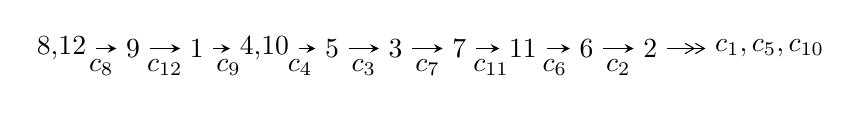
\begin{tikzpicture}[x=23pt, y=7pt]
	% node
	\node (A0) at (-1/8, 0) {8,12};
	\node (A1) at (1, 0) {9};
	\node (A2) at (2, 0) {1};
	\node (A3) at (49/16, 0) {4,10};
	\node (A4) at (33/8, 0) {5};
	\node (A5) at (41/8, 0) {3};
	\node (A6) at (49/8, 0) {7};
	\node (A7) at (57/8, 0) {11};
	\node (A8) at (65/8, 0) {6};
	\node (A9) at (73/8, 0) {2};
	\node (C1) at (1/2, -1) {$c_{8}$};
	\node (C2) at (3/2, -1) {$c_{12}$};
	\node (C3) at (5/2, -1) {$c_{9}$};
	\node (C4) at (29/8, -1) {$c_{4}$};
	\node (C5) at (37/8, -1) {$c_{3}$};
	\node (C6) at (45/8, -1) {$c_{7}$};
	\node (C7) at (53/8, -1) {$c_{11}$};
	\node (C8) at (61/8, -1) {$c_{6}$};
	\node (C9) at (69/8, -1) {$c_{2}$};
	\node (A10) at (11, 0) {$c_{1},c_{5},c_{10}$};

	% edge
	\draw[->,>=stealth]	
	(A0) edge (A1) (A1) edge (A2) (A2) edge (A3) (A3) edge (A4) (A4) edge (A5) (A5) edge (A6) (A6) edge (A7) (A7) edge (A8) (A8) edge (A9) ;
	\draw[->>,>={angle 60}]	
	(A9) edge (A10);
\end{tikzpicture} \\ 

\end{tabular} \\

\footnotetext{
The image of knot diagram is generated by the software ``\textbf{Draw programme}" developed by Andrew Bartholomew(\url{http://www.layer8.co.uk/maths/draw/index.htm\#Running-draw}), where we modified some parts for our purpose(\url{https://github.com/CATsTAILs/LinksPainter}).
}\phantom \\ \newline 
\centering \textbf{Ideals for irreducible components\footnotemark of $X_{\text{par}}$} 
 
\begin{align*}
I^u_{1}&=\langle 
-4.96183\times10^{229} u^{98}-1.54116\times10^{230} u^{97}+\cdots+5.52314\times10^{228} b+3.65483\times10^{230},\\
\phantom{I^u_{1}}&\phantom{= \langle  }2.26754\times10^{231} u^{98}+7.18353\times10^{231} u^{97}+\cdots+5.52314\times10^{228} a-1.28816\times10^{232},\;u^{99}+3 u^{98}+\cdots-20 u+1\rangle \\
I^u_{2}&=\langle 
187 u^{15}-333 u^{14}+\cdots+71 b-316,\;68 u^{15}-205 u^{14}+\cdots+71 a-457,\;u^{16}-2 u^{15}+\cdots-6 u-1\rangle \\
\\
\end{align*}
\raggedright * 2 irreducible components of $\dim_{\mathbb{C}}=0$, with total 115 representations.\\
\footnotetext{All coefficients of polynomials are rational numbers. But the coefficients are sometimes approximated in decimal forms when there is not enough margin.}
\newpage
\renewcommand{\arraystretch}{1}
\centering \section*{I. $I^u_{1}= \langle -4.96\times10^{229} u^{98}-1.54\times10^{230} u^{97}+\cdots+5.52\times10^{228} b+3.65\times10^{230},\;2.27\times10^{231} u^{98}+7.18\times10^{231} u^{97}+\cdots+5.52\times10^{228} a-1.29\times10^{232},\;u^{99}+3 u^{98}+\cdots-20 u+1 \rangle$}
\flushleft \textbf{(i) Arc colorings}\\
\begin{tabular}{m{7pt} m{180pt} m{7pt} m{180pt} }
\flushright $a_{8}=$&$\begin{pmatrix}1\\0\end{pmatrix}$ \\
\flushright $a_{12}=$&$\begin{pmatrix}0\\u\end{pmatrix}$ \\
\flushright $a_{9}=$&$\begin{pmatrix}1\\- u^2\end{pmatrix}$ \\
\flushright $a_{1}=$&$\begin{pmatrix}u\\- u^3+u\end{pmatrix}$ \\
\flushright $a_{4}=$&$\begin{pmatrix}-410.552 u^{98}-1300.62 u^{97}+\cdots-33247.6 u+2332.30\\8.98371 u^{98}+27.9038 u^{97}+\cdots+851.061 u-66.1730\end{pmatrix}$ \\
\flushright $a_{10}=$&$\begin{pmatrix}- u^2+1\\u^4-2 u^2\end{pmatrix}$ \\
\flushright $a_{5}=$&$\begin{pmatrix}-426.755 u^{98}-1351.65 u^{97}+\cdots-34375.4 u+2404.93\\10.5930 u^{98}+32.6000 u^{97}+\cdots+948.262 u-72.6394\end{pmatrix}$ \\
\flushright $a_{3}=$&$\begin{pmatrix}-401.569 u^{98}-1272.72 u^{97}+\cdots-32396.5 u+2266.13\\8.98371 u^{98}+27.9038 u^{97}+\cdots+851.061 u-66.1730\end{pmatrix}$ \\
\flushright $a_{7}=$&$\begin{pmatrix}-190.944 u^{98}-604.011 u^{97}+\cdots-15994.4 u+1130.44\\38.9398 u^{98}+120.404 u^{97}+\cdots+3169.91 u-230.155\end{pmatrix}$ \\
\flushright $a_{11}=$&$\begin{pmatrix}-525.908 u^{98}-1667.80 u^{97}+\cdots-44094.0 u+3123.09\\22.7841 u^{98}+74.5759 u^{97}+\cdots+2125.65 u-154.013\end{pmatrix}$ \\
\flushright $a_{6}=$&$\begin{pmatrix}847.939 u^{98}+2682.65 u^{97}+\cdots+70075.5 u-4962.87\\43.6317 u^{98}+137.298 u^{97}+\cdots+3675.73 u-263.137\end{pmatrix}$ \\
\flushright $a_{2}=$&$\begin{pmatrix}-839.291 u^{98}-2655.52 u^{97}+\cdots-69413.1 u+4916.87\\-43.1587 u^{98}-135.565 u^{97}+\cdots-3615.21 u+258.560\end{pmatrix}$\\&\end{tabular}
\flushleft \textbf{(ii) Obstruction class $= -1$}\\~\\
\flushleft \textbf{(iii) Cusp Shapes $= -84.5894 u^{98}-274.529 u^{97}+\cdots-7761.27 u+561.078$}\\~\\
\newpage\renewcommand{\arraystretch}{1}
\flushleft \textbf{(iv) u-Polynomials at the component}\newline \\
\begin{tabular}{m{50pt}|m{274pt}}
Crossings & \hspace{64pt}u-Polynomials at each crossing \\
\hline $$\begin{aligned}c_{1}\end{aligned}$$&$\begin{aligned}
&u^{99}- u^{98}+\cdots-420367 u-86857
\end{aligned}$\\
\hline $$\begin{aligned}c_{2},c_{5}\end{aligned}$$&$\begin{aligned}
&u^{99}-30 u^{97}+\cdots+7 u-1
\end{aligned}$\\
\hline $$\begin{aligned}c_{3},c_{7}\end{aligned}$$&$\begin{aligned}
&u^{99}-2 u^{98}+\cdots-303 u+61
\end{aligned}$\\
\hline $$\begin{aligned}c_{4},c_{10}\end{aligned}$$&$\begin{aligned}
&u^{99}- u^{98}+\cdots-39 u+937
\end{aligned}$\\
\hline $$\begin{aligned}c_{6},c_{11}\end{aligned}$$&$\begin{aligned}
&u^{99}+u^{98}+\cdots-5 u+1
\end{aligned}$\\
\hline $$\begin{aligned}c_{8},c_{9},c_{12}\end{aligned}$$&$\begin{aligned}
&u^{99}-3 u^{98}+\cdots-20 u-1
\end{aligned}$\\
\hline
\end{tabular}\\~\\
\newpage\renewcommand{\arraystretch}{1}
\flushleft \textbf{(v) Riley Polynomials at the component}\newline \\
\begin{tabular}{m{50pt}|m{274pt}}
Crossings & \hspace{64pt}Riley Polynomials at each crossing \\
\hline $$\begin{aligned}c_{1}\end{aligned}$$&$\begin{aligned}
&y^{99}+29 y^{98}+\cdots+12950485171 y-7544138449
\end{aligned}$\\
\hline $$\begin{aligned}c_{2},c_{5}\end{aligned}$$&$\begin{aligned}
&y^{99}-60 y^{98}+\cdots+125 y-1
\end{aligned}$\\
\hline $$\begin{aligned}c_{3},c_{7}\end{aligned}$$&$\begin{aligned}
&y^{99}-60 y^{98}+\cdots+178673 y-3721
\end{aligned}$\\
\hline $$\begin{aligned}c_{4},c_{10}\end{aligned}$$&$\begin{aligned}
&y^{99}-83 y^{98}+\cdots+55082129 y-877969
\end{aligned}$\\
\hline $$\begin{aligned}c_{6},c_{11}\end{aligned}$$&$\begin{aligned}
&y^{99}-67 y^{98}+\cdots+147 y-1
\end{aligned}$\\
\hline $$\begin{aligned}c_{8},c_{9},c_{12}\end{aligned}$$&$\begin{aligned}
&y^{99}-107 y^{98}+\cdots+92 y-1
\end{aligned}$\\
\hline
\end{tabular}\\~\\
\newpage\flushleft \textbf{(vi) Complex Volumes and Cusp Shapes}
$$\begin{array}{c|c|c}  
\text{Solutions to }I^u_{1}& \I (\text{vol} + \sqrt{-1}CS) & \text{Cusp shape}\\
 \hline 
\begin{aligned}
u &= -0.740716 + 0.660134 I \\
a &= -0.418260 - 0.619628 I \\
b &= \phantom{-}1.051910 - 0.341857 I\end{aligned}
 & -2.64189 + 2.94712 I & \phantom{-0.000000 } 0 \\ \hline\begin{aligned}
u &= -0.740716 - 0.660134 I \\
a &= -0.418260 + 0.619628 I \\
b &= \phantom{-}1.051910 + 0.341857 I\end{aligned}
 & -2.64189 - 2.94712 I & \phantom{-0.000000 } 0 \\ \hline\begin{aligned}
u &= \phantom{-}0.936978 + 0.373185 I \\
a &= \phantom{-}0.652429 - 0.083726 I \\
b &= \phantom{-}0.041110 + 0.447920 I\end{aligned}
 & \phantom{-}6.51007 + 1.78657 I & \phantom{-0.000000 } 0 \\ \hline\begin{aligned}
u &= \phantom{-}0.936978 - 0.373185 I \\
a &= \phantom{-}0.652429 + 0.083726 I \\
b &= \phantom{-}0.041110 - 0.447920 I\end{aligned}
 & \phantom{-}6.51007 - 1.78657 I & \phantom{-0.000000 } 0 \\ \hline\begin{aligned}
u &= -0.101390 + 0.907405 I \\
a &= -0.846291 + 0.518149 I \\
b &= -0.597672 + 0.210243 I\end{aligned}
 & \phantom{-}1.37944 - 3.96642 I & \phantom{-0.000000 } 0 \\ \hline\begin{aligned}
u &= -0.101390 - 0.907405 I \\
a &= -0.846291 - 0.518149 I \\
b &= -0.597672 - 0.210243 I\end{aligned}
 & \phantom{-}1.37944 + 3.96642 I & \phantom{-0.000000 } 0 \\ \hline\begin{aligned}
u &= \phantom{-}0.651492 + 0.873430 I \\
a &= -0.411850 - 0.833116 I \\
b &= -1.246290 + 0.572677 I\end{aligned}
 & \phantom{-}0.38169 + 13.20470 I & \phantom{-0.000000 } 0 \\ \hline\begin{aligned}
u &= \phantom{-}0.651492 - 0.873430 I \\
a &= -0.411850 + 0.833116 I \\
b &= -1.246290 - 0.572677 I\end{aligned}
 & \phantom{-}0.38169 - 13.20470 I & \phantom{-0.000000 } 0 \\ \hline\begin{aligned}
u &= \phantom{-}0.905341\phantom{ +0.000000I} \\
a &= \phantom{-}0.739427\phantom{ +0.000000I} \\
b &= -1.62008\phantom{ +0.000000I}\end{aligned}
 & -7.39496\phantom{ +0.000000I} & \phantom{-0.000000 } 0 \\ \hline\begin{aligned}
u &= -0.561511 + 0.671788 I \\
a &= \phantom{-}0.20921 - 1.46205 I \\
b &= \phantom{-}1.200880 + 0.244534 I\end{aligned}
 & -3.26168 - 6.50239 I & \phantom{-0.000000 } 0\\
 \hline 
 \end{array}$$\newpage$$\begin{array}{c|c|c}  
\text{Solutions to }I^u_{1}& \I (\text{vol} + \sqrt{-1}CS) & \text{Cusp shape}\\
 \hline 
\begin{aligned}
u &= -0.561511 - 0.671788 I \\
a &= \phantom{-}0.20921 + 1.46205 I \\
b &= \phantom{-}1.200880 - 0.244534 I\end{aligned}
 & -3.26168 + 6.50239 I & \phantom{-0.000000 } 0 \\ \hline\begin{aligned}
u &= -0.380686 + 0.733717 I \\
a &= \phantom{-}0.574255 - 0.663992 I \\
b &= \phantom{-}1.254820 + 0.607843 I\end{aligned}
 & -3.66994 - 7.66735 I & \phantom{-0.000000 } 0 \\ \hline\begin{aligned}
u &= -0.380686 - 0.733717 I \\
a &= \phantom{-}0.574255 + 0.663992 I \\
b &= \phantom{-}1.254820 - 0.607843 I\end{aligned}
 & -3.66994 + 7.66735 I & \phantom{-0.000000 } 0 \\ \hline\begin{aligned}
u &= -0.496979 + 0.655506 I \\
a &= \phantom{-}0.281407 - 0.243550 I \\
b &= \phantom{-}1.269220 - 0.043803 I\end{aligned}
 & -3.47162 + 1.98683 I & \phantom{-0.000000 } 0 \\ \hline\begin{aligned}
u &= -0.496979 - 0.655506 I \\
a &= \phantom{-}0.281407 + 0.243550 I \\
b &= \phantom{-}1.269220 + 0.043803 I\end{aligned}
 & -3.47162 - 1.98683 I & \phantom{-0.000000 } 0 \\ \hline\begin{aligned}
u &= \phantom{-}0.818206\phantom{ +0.000000I} \\
a &= \phantom{-}2.13556\phantom{ +0.000000I} \\
b &= -1.09275\phantom{ +0.000000I}\end{aligned}
 & \phantom{-}4.08306\phantom{ +0.000000I} & \phantom{-0.000000 } 0 \\ \hline\begin{aligned}
u &= \phantom{-}0.662406 + 0.453421 I \\
a &= -0.235423 + 0.522548 I \\
b &= -0.064412 - 1.004580 I\end{aligned}
 & \phantom{-}3.86389 + 7.67810 I & \phantom{-0.000000 } 0 \\ \hline\begin{aligned}
u &= \phantom{-}0.662406 - 0.453421 I \\
a &= -0.235423 - 0.522548 I \\
b &= -0.064412 + 1.004580 I\end{aligned}
 & \phantom{-}3.86389 - 7.67810 I & \phantom{-0.000000 } 0 \\ \hline\begin{aligned}
u &= \phantom{-}0.523831 + 1.105700 I \\
a &= -0.105946 - 0.261595 I \\
b &= -1.031180 - 0.382990 I\end{aligned}
 & -0.13947 - 6.93665 I & \phantom{-0.000000 } 0 \\ \hline\begin{aligned}
u &= \phantom{-}0.523831 - 1.105700 I \\
a &= -0.105946 + 0.261595 I \\
b &= -1.031180 + 0.382990 I\end{aligned}
 & -0.13947 + 6.93665 I & \phantom{-0.000000 } 0\\
 \hline 
 \end{array}$$\newpage$$\begin{array}{c|c|c}  
\text{Solutions to }I^u_{1}& \I (\text{vol} + \sqrt{-1}CS) & \text{Cusp shape}\\
 \hline 
\begin{aligned}
u &= \phantom{-}0.450653 + 0.606011 I \\
a &= -0.110925 - 1.084860 I \\
b &= -1.283860 + 0.169700 I\end{aligned}
 & -7.12534 + 2.00701 I & \phantom{-0.000000 } 0 \\ \hline\begin{aligned}
u &= \phantom{-}0.450653 - 0.606011 I \\
a &= -0.110925 + 1.084860 I \\
b &= -1.283860 - 0.169700 I\end{aligned}
 & -7.12534 - 2.00701 I & \phantom{-0.000000 } 0 \\ \hline\begin{aligned}
u &= -0.365780 + 0.654899 I \\
a &= -0.639028 + 0.869862 I \\
b &= -0.365840 - 0.469149 I\end{aligned}
 & \phantom{-}1.00378 - 3.95796 I & \phantom{-0.000000 } 0 \\ \hline\begin{aligned}
u &= -0.365780 - 0.654899 I \\
a &= -0.639028 - 0.869862 I \\
b &= -0.365840 + 0.469149 I\end{aligned}
 & \phantom{-}1.00378 + 3.95796 I & \phantom{-0.000000 } 0 \\ \hline\begin{aligned}
u &= -0.656614 + 0.362229 I \\
a &= \phantom{-}0.0542687 + 0.0829791 I \\
b &= -0.631447 + 0.366281 I\end{aligned}
 & \phantom{-}1.010570 + 0.037156 I & \phantom{-0.000000 } 0 \\ \hline\begin{aligned}
u &= -0.656614 - 0.362229 I \\
a &= \phantom{-}0.0542687 - 0.0829791 I \\
b &= -0.631447 - 0.366281 I\end{aligned}
 & \phantom{-}1.010570 - 0.037156 I & \phantom{-0.000000 } 0 \\ \hline\begin{aligned}
u &= -0.347291 + 0.663112 I \\
a &= -1.069160 + 0.749279 I \\
b &= -0.979170 - 0.487234 I\end{aligned}
 & -0.08310 - 3.86265 I & \phantom{-0.000000 } 0 \\ \hline\begin{aligned}
u &= -0.347291 - 0.663112 I \\
a &= -1.069160 - 0.749279 I \\
b &= -0.979170 + 0.487234 I\end{aligned}
 & -0.08310 + 3.86265 I & \phantom{-0.000000 } 0 \\ \hline\begin{aligned}
u &= -0.391345 + 0.627891 I \\
a &= -1.11464 + 1.09083 I \\
b &= -0.966274 - 0.492186 I\end{aligned}
 & -0.05253 - 3.83284 I & \phantom{-0.000000 } 0 \\ \hline\begin{aligned}
u &= -0.391345 - 0.627891 I \\
a &= -1.11464 - 1.09083 I \\
b &= -0.966274 + 0.492186 I\end{aligned}
 & -0.05253 + 3.83284 I & \phantom{-0.000000 } 0\\
 \hline 
 \end{array}$$\newpage$$\begin{array}{c|c|c}  
\text{Solutions to }I^u_{1}& \I (\text{vol} + \sqrt{-1}CS) & \text{Cusp shape}\\
 \hline 
\begin{aligned}
u &= -1.271100 + 0.059881 I \\
a &= -0.26161 + 1.40515 I \\
b &= -0.440116 - 0.157984 I\end{aligned}
 & \phantom{-}2.03091 + 1.52575 I & \phantom{-0.000000 } 0 \\ \hline\begin{aligned}
u &= -1.271100 - 0.059881 I \\
a &= -0.26161 - 1.40515 I \\
b &= -0.440116 + 0.157984 I\end{aligned}
 & \phantom{-}2.03091 - 1.52575 I & \phantom{-0.000000 } 0 \\ \hline\begin{aligned}
u &= \phantom{-}0.722291 + 0.051213 I \\
a &= -1.62389 + 0.90390 I \\
b &= \phantom{-}0.804246 - 0.598002 I\end{aligned}
 & \phantom{-}1.59199 - 1.46670 I & \phantom{-0.000000 } 0 \\ \hline\begin{aligned}
u &= \phantom{-}0.722291 - 0.051213 I \\
a &= -1.62389 - 0.90390 I \\
b &= \phantom{-}0.804246 + 0.598002 I\end{aligned}
 & \phantom{-}1.59199 + 1.46670 I & \phantom{-0.000000 } 0 \\ \hline\begin{aligned}
u &= -0.485156 + 0.504923 I \\
a &= \phantom{-}0.377985 - 0.473286 I \\
b &= -0.316264 + 0.537966 I\end{aligned}
 & \phantom{-}1.47556 + 0.10354 I & \phantom{-0.000000 } 0 \\ \hline\begin{aligned}
u &= -0.485156 - 0.504923 I \\
a &= \phantom{-}0.377985 + 0.473286 I \\
b &= -0.316264 - 0.537966 I\end{aligned}
 & \phantom{-}1.47556 - 0.10354 I & \phantom{-0.000000 } 0 \\ \hline\begin{aligned}
u &= \phantom{-}0.652970 + 1.136450 I \\
a &= \phantom{-}0.431392 + 0.440530 I \\
b &= \phantom{-}1.072920 - 0.439287 I\end{aligned}
 & \phantom{-}4.12271 + 5.39603 I & \phantom{-0.000000 } 0 \\ \hline\begin{aligned}
u &= \phantom{-}0.652970 - 1.136450 I \\
a &= \phantom{-}0.431392 - 0.440530 I \\
b &= \phantom{-}1.072920 + 0.439287 I\end{aligned}
 & \phantom{-}4.12271 - 5.39603 I & \phantom{-0.000000 } 0 \\ \hline\begin{aligned}
u &= -0.685910\phantom{ +0.000000I} \\
a &= -0.246736\phantom{ +0.000000I} \\
b &= -0.433093\phantom{ +0.000000I}\end{aligned}
 & \phantom{-}0.890789\phantom{ +0.000000I} & \phantom{-0.000000 } 0 \\ \hline\begin{aligned}
u &= \phantom{-}1.39035\phantom{ +0.000000I} \\
a &= \phantom{-}3.75335\phantom{ +0.000000I} \\
b &= -3.80795\phantom{ +0.000000I}\end{aligned}
 & \phantom{-}5.21323\phantom{ +0.000000I} & \phantom{-0.000000 } 0\\
 \hline 
 \end{array}$$\newpage$$\begin{array}{c|c|c}  
\text{Solutions to }I^u_{1}& \I (\text{vol} + \sqrt{-1}CS) & \text{Cusp shape}\\
 \hline 
\begin{aligned}
u &= \phantom{-}1.399680 + 0.087417 I \\
a &= -0.38568 - 1.67583 I \\
b &= \phantom{-}0.558612 + 0.259158 I\end{aligned}
 & \phantom{-}5.78712 + 6.53835 I & \phantom{-0.000000 } 0 \\ \hline\begin{aligned}
u &= \phantom{-}1.399680 - 0.087417 I \\
a &= -0.38568 + 1.67583 I \\
b &= \phantom{-}0.558612 - 0.259158 I\end{aligned}
 & \phantom{-}5.78712 - 6.53835 I & \phantom{-0.000000 } 0 \\ \hline\begin{aligned}
u &= -1.400530 + 0.115235 I \\
a &= -0.38152 - 1.52179 I \\
b &= \phantom{-}0.782265 + 0.573377 I\end{aligned}
 & \phantom{-}3.64494 - 2.28231 I & \phantom{-0.000000 } 0 \\ \hline\begin{aligned}
u &= -1.400530 - 0.115235 I \\
a &= -0.38152 + 1.52179 I \\
b &= \phantom{-}0.782265 - 0.573377 I\end{aligned}
 & \phantom{-}3.64494 + 2.28231 I & \phantom{-0.000000 } 0 \\ \hline\begin{aligned}
u &= -1.41818 + 0.01985 I \\
a &= -1.78789 - 3.09256 I \\
b &= \phantom{-}2.08833 + 2.72201 I\end{aligned}
 & \phantom{-}4.68486 + 0.26157 I & \phantom{-0.000000 } 0 \\ \hline\begin{aligned}
u &= -1.41818 - 0.01985 I \\
a &= -1.78789 + 3.09256 I \\
b &= \phantom{-}2.08833 - 2.72201 I\end{aligned}
 & \phantom{-}4.68486 - 0.26157 I & \phantom{-0.000000 } 0 \\ \hline\begin{aligned}
u &= \phantom{-}1.40357 + 0.23061 I \\
a &= -0.008833 + 0.931264 I \\
b &= \phantom{-}1.236100 - 0.413960 I\end{aligned}
 & \phantom{-}3.29811 + 2.26423 I & \phantom{-0.000000 } 0 \\ \hline\begin{aligned}
u &= \phantom{-}1.40357 - 0.23061 I \\
a &= -0.008833 - 0.931264 I \\
b &= \phantom{-}1.236100 + 0.413960 I\end{aligned}
 & \phantom{-}3.29811 - 2.26423 I & \phantom{-0.000000 } 0 \\ \hline\begin{aligned}
u &= \phantom{-}1.43957 + 0.02655 I \\
a &= -0.651757 - 0.245845 I \\
b &= \phantom{-}1.316080 + 0.146662 I\end{aligned}
 & \phantom{-}3.35235 + 0.02455 I & \phantom{-0.000000 } 0 \\ \hline\begin{aligned}
u &= \phantom{-}1.43957 - 0.02655 I \\
a &= -0.651757 + 0.245845 I \\
b &= \phantom{-}1.316080 - 0.146662 I\end{aligned}
 & \phantom{-}3.35235 - 0.02455 I & \phantom{-0.000000 } 0\\
 \hline 
 \end{array}$$\newpage$$\begin{array}{c|c|c}  
\text{Solutions to }I^u_{1}& \I (\text{vol} + \sqrt{-1}CS) & \text{Cusp shape}\\
 \hline 
\begin{aligned}
u &= \phantom{-}1.43958 + 0.09510 I \\
a &= \phantom{-}0.62498 + 1.27990 I \\
b &= -0.599662 - 0.585723 I\end{aligned}
 & \phantom{-}7.52065 + 1.93273 I & \phantom{-0.000000 } 0 \\ \hline\begin{aligned}
u &= \phantom{-}1.43958 - 0.09510 I \\
a &= \phantom{-}0.62498 - 1.27990 I \\
b &= -0.599662 + 0.585723 I\end{aligned}
 & \phantom{-}7.52065 - 1.93273 I & \phantom{-0.000000 } 0 \\ \hline\begin{aligned}
u &= -1.45637 + 0.00770 I \\
a &= \phantom{-}0.039120 + 1.009860 I \\
b &= -1.359020 - 0.383649 I\end{aligned}
 & \phantom{-}9.19651 - 0.99992 I & \phantom{-0.000000 } 0 \\ \hline\begin{aligned}
u &= -1.45637 - 0.00770 I \\
a &= \phantom{-}0.039120 - 1.009860 I \\
b &= -1.359020 + 0.383649 I\end{aligned}
 & \phantom{-}9.19651 + 0.99992 I & \phantom{-0.000000 } 0 \\ \hline\begin{aligned}
u &= -1.46744 + 0.01290 I \\
a &= -0.05298 - 1.79361 I \\
b &= \phantom{-}1.117730 + 0.579902 I\end{aligned}
 & \phantom{-}7.50489 - 5.71904 I & \phantom{-0.000000 } 0 \\ \hline\begin{aligned}
u &= -1.46744 - 0.01290 I \\
a &= -0.05298 + 1.79361 I \\
b &= \phantom{-}1.117730 - 0.579902 I\end{aligned}
 & \phantom{-}7.50489 + 5.71904 I & \phantom{-0.000000 } 0 \\ \hline\begin{aligned}
u &= \phantom{-}1.45767 + 0.24111 I \\
a &= -0.47894 + 1.68889 I \\
b &= \phantom{-}1.36486 - 0.89980 I\end{aligned}
 & \phantom{-}2.25200 + 11.14920 I & \phantom{-0.000000 } 0 \\ \hline\begin{aligned}
u &= \phantom{-}1.45767 - 0.24111 I \\
a &= -0.47894 - 1.68889 I \\
b &= \phantom{-}1.36486 + 0.89980 I\end{aligned}
 & \phantom{-}2.25200 - 11.14920 I & \phantom{-0.000000 } 0 \\ \hline\begin{aligned}
u &= \phantom{-}1.46515 + 0.22421 I \\
a &= \phantom{-}0.16687 - 1.54702 I \\
b &= -1.166860 + 0.696988 I\end{aligned}
 & \phantom{-}5.81806 + 7.08117 I & \phantom{-0.000000 } 0 \\ \hline\begin{aligned}
u &= \phantom{-}1.46515 - 0.22421 I \\
a &= \phantom{-}0.16687 + 1.54702 I \\
b &= -1.166860 - 0.696988 I\end{aligned}
 & \phantom{-}5.81806 - 7.08117 I & \phantom{-0.000000 } 0\\
 \hline 
 \end{array}$$\newpage$$\begin{array}{c|c|c}  
\text{Solutions to }I^u_{1}& \I (\text{vol} + \sqrt{-1}CS) & \text{Cusp shape}\\
 \hline 
\begin{aligned}
u &= -1.46946 + 0.19795 I \\
a &= \phantom{-}0.74012 + 1.33954 I \\
b &= -1.167030 - 0.485918 I\end{aligned}
 & -0.91244 - 4.91882 I & \phantom{-0.000000 } 0 \\ \hline\begin{aligned}
u &= -1.46946 - 0.19795 I \\
a &= \phantom{-}0.74012 - 1.33954 I \\
b &= -1.167030 + 0.485918 I\end{aligned}
 & -0.91244 + 4.91882 I & \phantom{-0.000000 } 0 \\ \hline\begin{aligned}
u &= \phantom{-}1.39576 + 0.53376 I \\
a &= \phantom{-}0.189616 + 0.503312 I \\
b &= \phantom{-}0.520698 + 0.028555 I\end{aligned}
 & \phantom{-}6.45396 + 2.02499 I & \phantom{-0.000000 } 0 \\ \hline\begin{aligned}
u &= \phantom{-}1.39576 - 0.53376 I \\
a &= \phantom{-}0.189616 - 0.503312 I \\
b &= \phantom{-}0.520698 - 0.028555 I\end{aligned}
 & \phantom{-}6.45396 - 2.02499 I & \phantom{-0.000000 } 0 \\ \hline\begin{aligned}
u &= \phantom{-}1.48191 + 0.26155 I \\
a &= -0.08251 - 1.46403 I \\
b &= -0.680631 + 0.669773 I\end{aligned}
 & \phantom{-}6.98172 + 7.44981 I & \phantom{-0.000000 } 0 \\ \hline\begin{aligned}
u &= \phantom{-}1.48191 - 0.26155 I \\
a &= -0.08251 + 1.46403 I \\
b &= -0.680631 - 0.669773 I\end{aligned}
 & \phantom{-}6.98172 - 7.44981 I & \phantom{-0.000000 } 0 \\ \hline\begin{aligned}
u &= \phantom{-}1.51340 + 0.06368 I \\
a &= \phantom{-}0.519798 + 1.055950 I \\
b &= -0.410844 - 0.828111 I\end{aligned}
 & \phantom{-}7.91657 + 1.31701 I & \phantom{-0.000000 } 0 \\ \hline\begin{aligned}
u &= \phantom{-}1.51340 - 0.06368 I \\
a &= \phantom{-}0.519798 - 1.055950 I \\
b &= -0.410844 + 0.828111 I\end{aligned}
 & \phantom{-}7.91657 - 1.31701 I & \phantom{-0.000000 } 0 \\ \hline\begin{aligned}
u &= \phantom{-}1.50217 + 0.21346 I \\
a &= \phantom{-}0.18452 - 1.71021 I \\
b &= -1.048460 + 0.615613 I\end{aligned}
 & \phantom{-}6.22115 + 6.89414 I & \phantom{-0.000000 } 0 \\ \hline\begin{aligned}
u &= \phantom{-}1.50217 - 0.21346 I \\
a &= \phantom{-}0.18452 + 1.71021 I \\
b &= -1.048460 - 0.615613 I\end{aligned}
 & \phantom{-}6.22115 - 6.89414 I & \phantom{-0.000000 } 0\\
 \hline 
 \end{array}$$\newpage$$\begin{array}{c|c|c}  
\text{Solutions to }I^u_{1}& \I (\text{vol} + \sqrt{-1}CS) & \text{Cusp shape}\\
 \hline 
\begin{aligned}
u &= -1.55288 + 0.15662 I \\
a &= \phantom{-}0.32381 - 1.59916 I \\
b &= -0.24255 + 1.46889 I\end{aligned}
 & \phantom{-}11.1954 - 10.0068 I & \phantom{-0.000000 } 0 \\ \hline\begin{aligned}
u &= -1.55288 - 0.15662 I \\
a &= \phantom{-}0.32381 + 1.59916 I \\
b &= -0.24255 - 1.46889 I\end{aligned}
 & \phantom{-}11.1954 + 10.0068 I & \phantom{-0.000000 } 0 \\ \hline\begin{aligned}
u &= -0.025265 + 0.430438 I \\
a &= \phantom{-}1.50952 + 1.48306 I \\
b &= \phantom{-}0.668301 + 0.118557 I\end{aligned}
 & -1.202850 + 0.483660 I & -4.55970 + 1.18319 I \\ \hline\begin{aligned}
u &= -0.025265 - 0.430438 I \\
a &= \phantom{-}1.50952 - 1.48306 I \\
b &= \phantom{-}0.668301 - 0.118557 I\end{aligned}
 & -1.202850 - 0.483660 I & -4.55970 - 1.18319 I \\ \hline\begin{aligned}
u &= \phantom{-}1.55291 + 0.22303 I \\
a &= -0.62785 + 1.55930 I \\
b &= \phantom{-}1.104160 - 0.431801 I\end{aligned}
 & \phantom{-}3.73273 + 9.79679 I & \phantom{-0.000000 } 0 \\ \hline\begin{aligned}
u &= \phantom{-}1.55291 - 0.22303 I \\
a &= -0.62785 - 1.55930 I \\
b &= \phantom{-}1.104160 + 0.431801 I\end{aligned}
 & \phantom{-}3.73273 - 9.79679 I & \phantom{-0.000000 } 0 \\ \hline\begin{aligned}
u &= -1.59493 + 0.15891 I \\
a &= -0.173089 + 1.219070 I \\
b &= \phantom{-}0.227269 - 1.134870 I\end{aligned}
 & \phantom{-}14.7475 - 4.1486 I & \phantom{-0.000000 } 0 \\ \hline\begin{aligned}
u &= -1.59493 - 0.15891 I \\
a &= -0.173089 - 1.219070 I \\
b &= \phantom{-}0.227269 + 1.134870 I\end{aligned}
 & \phantom{-}14.7475 + 4.1486 I & \phantom{-0.000000 } 0 \\ \hline\begin{aligned}
u &= -0.263578 + 0.291460 I \\
a &= -0.327340 + 0.152958 I \\
b &= -0.905011 + 1.083140 I\end{aligned}
 & \phantom{-}0.448592 + 0.918224 I & \phantom{-}4.55809 + 12.61038 I \\ \hline\begin{aligned}
u &= -0.263578 - 0.291460 I \\
a &= -0.327340 - 0.152958 I \\
b &= -0.905011 - 1.083140 I\end{aligned}
 & \phantom{-}0.448592 - 0.918224 I & \phantom{-}4.55809 - 12.61038 I\\
 \hline 
 \end{array}$$\newpage$$\begin{array}{c|c|c}  
\text{Solutions to }I^u_{1}& \I (\text{vol} + \sqrt{-1}CS) & \text{Cusp shape}\\
 \hline 
\begin{aligned}
u &= -1.58652 + 0.29743 I \\
a &= \phantom{-}0.36085 + 1.51692 I \\
b &= -1.36467 - 0.75652 I\end{aligned}
 & \phantom{-}7.6756 - 17.5314 I & \phantom{-0.000000 } 0 \\ \hline\begin{aligned}
u &= -1.58652 - 0.29743 I \\
a &= \phantom{-}0.36085 - 1.51692 I \\
b &= -1.36467 + 0.75652 I\end{aligned}
 & \phantom{-}7.6756 + 17.5314 I & \phantom{-0.000000 } 0 \\ \hline\begin{aligned}
u &= -1.62548 + 0.07252 I \\
a &= -0.690393 - 0.963420 I \\
b &= \phantom{-}0.344934 + 0.690280 I\end{aligned}
 & \phantom{-}9.73410 + 0.77955 I & \phantom{-0.000000 } 0 \\ \hline\begin{aligned}
u &= -1.62548 - 0.07252 I \\
a &= -0.690393 + 0.963420 I \\
b &= \phantom{-}0.344934 - 0.690280 I\end{aligned}
 & \phantom{-}9.73410 - 0.77955 I & \phantom{-0.000000 } 0 \\ \hline\begin{aligned}
u &= -1.63242\phantom{ +0.000000I} \\
a &= \phantom{-}1.49914\phantom{ +0.000000I} \\
b &= -0.727141\phantom{ +0.000000I}\end{aligned}
 & \phantom{-}12.5284\phantom{ +0.000000I} & \phantom{-0.000000 } 0 \\ \hline\begin{aligned}
u &= \phantom{-}0.060339 + 0.361917 I \\
a &= \phantom{-}1.09542 + 1.69316 I \\
b &= \phantom{-}0.652611 - 0.069393 I\end{aligned}
 & -1.221060 + 0.471555 I & -5.19431 - 0.44409 I \\ \hline\begin{aligned}
u &= \phantom{-}0.060339 - 0.361917 I \\
a &= \phantom{-}1.09542 - 1.69316 I \\
b &= \phantom{-}0.652611 + 0.069393 I\end{aligned}
 & -1.221060 - 0.471555 I & -5.19431 + 0.44409 I \\ \hline\begin{aligned}
u &= -1.60187 + 0.33615 I \\
a &= -0.212049 - 1.278830 I \\
b &= \phantom{-}1.29576 + 0.66671 I\end{aligned}
 & \phantom{-}11.4391 - 10.5221 I & \phantom{-0.000000 } 0 \\ \hline\begin{aligned}
u &= -1.60187 - 0.33615 I \\
a &= -0.212049 + 1.278830 I \\
b &= \phantom{-}1.29576 - 0.66671 I\end{aligned}
 & \phantom{-}11.4391 + 10.5221 I & \phantom{-0.000000 } 0 \\ \hline\begin{aligned}
u &= \phantom{-}1.73495\phantom{ +0.000000I} \\
a &= -0.540652\phantom{ +0.000000I} \\
b &= \phantom{-}0.633937\phantom{ +0.000000I}\end{aligned}
 & \phantom{-}6.52917\phantom{ +0.000000I} & \phantom{-0.000000 } 0\\
 \hline 
 \end{array}$$\newpage$$\begin{array}{c|c|c}  
\text{Solutions to }I^u_{1}& \I (\text{vol} + \sqrt{-1}CS) & \text{Cusp shape}\\
 \hline 
\begin{aligned}
u &= -1.64465 + 0.57114 I \\
a &= -0.021397 + 0.670503 I \\
b &= -1.173420 - 0.398009 I\end{aligned}
 & \phantom{-}5.87495 - 2.46826 I & \phantom{-0.000000 } 0 \\ \hline\begin{aligned}
u &= -1.64465 - 0.57114 I \\
a &= -0.021397 - 0.670503 I \\
b &= -1.173420 + 0.398009 I\end{aligned}
 & \phantom{-}5.87495 + 2.46826 I & \phantom{-0.000000 } 0 \\ \hline\begin{aligned}
u &= \phantom{-}0.112870 + 0.195686 I \\
a &= \phantom{-}1.43436 + 0.89523 I \\
b &= \phantom{-}1.09114 - 1.27035 I\end{aligned}
 & -0.384516 - 0.802457 I & -4.4738 - 22.9416 I \\ \hline\begin{aligned}
u &= \phantom{-}0.112870 - 0.195686 I \\
a &= \phantom{-}1.43436 - 0.89523 I \\
b &= \phantom{-}1.09114 + 1.27035 I\end{aligned}
 & -0.384516 + 0.802457 I & -4.4738 + 22.9416 I \\ \hline\begin{aligned}
u &= \phantom{-}0.203707 + 0.028208 I \\
a &= \phantom{-}1.93686 - 8.64962 I \\
b &= \phantom{-}0.798444 + 0.440266 I\end{aligned}
 & \phantom{-}1.72855 - 5.65485 I & \phantom{-}9.03689 + 7.91182 I \\ \hline\begin{aligned}
u &= \phantom{-}0.203707 - 0.028208 I \\
a &= \phantom{-}1.93686 + 8.64962 I \\
b &= \phantom{-}0.798444 - 0.440266 I\end{aligned}
 & \phantom{-}1.72855 + 5.65485 I & \phantom{-}9.03689 - 7.91182 I \\ \hline\begin{aligned}
u &= \phantom{-}0.167144 + 0.003550 I \\
a &= -6.70304 - 5.00229 I \\
b &= -0.988849 + 0.291096 I\end{aligned}
 & \phantom{-}3.59911 + 0.92364 I & \phantom{-}5.70852 - 0.99827 I \\ \hline\begin{aligned}
u &= \phantom{-}0.167144 - 0.003550 I \\
a &= -6.70304 + 5.00229 I \\
b &= -0.988849 - 0.291096 I\end{aligned}
 & \phantom{-}3.59911 - 0.92364 I & \phantom{-}5.70852 + 0.99827 I \\ \hline\begin{aligned}
u &= -2.11117\phantom{ +0.000000I} \\
a &= \phantom{-}0.0909028\phantom{ +0.000000I} \\
b &= -0.618667\phantom{ +0.000000I}\end{aligned}
 & \phantom{-}8.75658\phantom{ +0.000000I} & \phantom{-0.000000 } 0\\
 \hline 
 \end{array}$$\newpage\newpage\renewcommand{\arraystretch}{1}
\centering \section*{II. $I^u_{2}= \langle 187 u^{15}-333 u^{14}+\cdots+71 b-316,\;68 u^{15}-205 u^{14}+\cdots+71 a-457,\;u^{16}-2 u^{15}+\cdots-6 u-1 \rangle$}
\flushleft \textbf{(i) Arc colorings}\\
\begin{tabular}{m{7pt} m{180pt} m{7pt} m{180pt} }
\flushright $a_{8}=$&$\begin{pmatrix}1\\0\end{pmatrix}$ \\
\flushright $a_{12}=$&$\begin{pmatrix}0\\u\end{pmatrix}$ \\
\flushright $a_{9}=$&$\begin{pmatrix}1\\- u^2\end{pmatrix}$ \\
\flushright $a_{1}=$&$\begin{pmatrix}u\\- u^3+u\end{pmatrix}$ \\
\flushright $a_{4}=$&$\begin{pmatrix}-0.957746 u^{15}+2.88732 u^{14}+\cdots+10.4648 u+6.43662\\-2.63380 u^{15}+4.69014 u^{14}+\cdots+11.0282 u+4.45070\end{pmatrix}$ \\
\flushright $a_{10}=$&$\begin{pmatrix}- u^2+1\\u^4-2 u^2\end{pmatrix}$ \\
\flushright $a_{5}=$&$\begin{pmatrix}-2.57746 u^{15}+5.87324 u^{14}+\cdots+18.6479 u+10.3662\\-2.50704 u^{15}+4.35211 u^{14}+\cdots+9.42254 u+3.76056\end{pmatrix}$ \\
\flushright $a_{3}=$&$\begin{pmatrix}-3.59155 u^{15}+7.57746 u^{14}+\cdots+21.4930 u+10.8873\\-2.63380 u^{15}+4.69014 u^{14}+\cdots+11.0282 u+4.45070\end{pmatrix}$ \\
\flushright $a_{7}=$&$\begin{pmatrix}0.267606 u^{15}-1.38028 u^{14}+\cdots-8.05634 u+1.09859\\0.676056 u^{15}+0.197183 u^{14}+\cdots+12.4366 u+4.98592\end{pmatrix}$ \\
\flushright $a_{11}=$&$\begin{pmatrix}1.46479 u^{15}-3.23944 u^{14}+\cdots-18.8873 u-3.19718\\-2.84507 u^{15}+3.25352 u^{14}+\cdots-1.29577 u+2.26761\end{pmatrix}$ \\
\flushright $a_{6}=$&$\begin{pmatrix}-2.63380 u^{15}+4.69014 u^{14}+\cdots+8.02817 u+6.45070\\-0.760563 u^{15}+0.0281690 u^{14}+\cdots-0.366197 u+1.14085\end{pmatrix}$ \\
\flushright $a_{2}=$&$\begin{pmatrix}-2 u^{15}+3 u^{14}+\cdots- u+2\\-0.323944 u^{15}+0.197183 u^{14}+\cdots+5.43662 u+1.98592\end{pmatrix}$\\&\end{tabular}
\flushleft \textbf{(ii) Obstruction class $= 1$}\\~\\
\flushleft \textbf{(iii) Cusp Shapes $= \frac{214}{71} u^{15}-\frac{973}{71} u^{14}+\cdots-\frac{3184}{71} u-\frac{250}{71}$}\\~\\
\newpage\renewcommand{\arraystretch}{1}
\flushleft \textbf{(iv) u-Polynomials at the component}\newline \\
\begin{tabular}{m{50pt}|m{274pt}}
Crossings & \hspace{64pt}u-Polynomials at each crossing \\
\hline $$\begin{aligned}c_{1}\end{aligned}$$&$\begin{aligned}
&u^{16}-6 u^{15}+\cdots-11 u+1
\end{aligned}$\\
\hline $$\begin{aligned}c_{2}\end{aligned}$$&$\begin{aligned}
&u^{16}+5 u^{15}+\cdots+3 u+1
\end{aligned}$\\
\hline $$\begin{aligned}c_{3}\end{aligned}$$&$\begin{aligned}
&u^{16}- u^{15}+\cdots- u-1
\end{aligned}$\\
\hline $$\begin{aligned}c_{4}\end{aligned}$$&$\begin{aligned}
&u^{16}-11 u^{14}+\cdots-9 u+1
\end{aligned}$\\
\hline $$\begin{aligned}c_{5}\end{aligned}$$&$\begin{aligned}
&u^{16}-5 u^{15}+\cdots-3 u+1
\end{aligned}$\\
\hline $$\begin{aligned}c_{6}\end{aligned}$$&$\begin{aligned}
&u^{16}+2 u^{15}+\cdots+u-1
\end{aligned}$\\
\hline $$\begin{aligned}c_{7}\end{aligned}$$&$\begin{aligned}
&u^{16}+u^{15}+\cdots+u-1
\end{aligned}$\\
\hline $$\begin{aligned}c_{8},c_{9}\end{aligned}$$&$\begin{aligned}
&u^{16}-2 u^{15}+\cdots-6 u-1
\end{aligned}$\\
\hline $$\begin{aligned}c_{10}\end{aligned}$$&$\begin{aligned}
&u^{16}-11 u^{14}+\cdots+9 u+1
\end{aligned}$\\
\hline $$\begin{aligned}c_{11}\end{aligned}$$&$\begin{aligned}
&u^{16}-2 u^{15}+\cdots- u-1
\end{aligned}$\\
\hline $$\begin{aligned}c_{12}\end{aligned}$$&$\begin{aligned}
&u^{16}+2 u^{15}+\cdots+6 u-1
\end{aligned}$\\
\hline
\end{tabular}\\~\\
\newpage\renewcommand{\arraystretch}{1}
\flushleft \textbf{(v) Riley Polynomials at the component}\newline \\
\begin{tabular}{m{50pt}|m{274pt}}
Crossings & \hspace{64pt}Riley Polynomials at each crossing \\
\hline $$\begin{aligned}c_{1}\end{aligned}$$&$\begin{aligned}
&y^{16}-2 y^{15}+\cdots-21 y+1
\end{aligned}$\\
\hline $$\begin{aligned}c_{2},c_{5}\end{aligned}$$&$\begin{aligned}
&y^{16}-15 y^{15}+\cdots-27 y+1
\end{aligned}$\\
\hline $$\begin{aligned}c_{3},c_{7}\end{aligned}$$&$\begin{aligned}
&y^{16}-19 y^{15}+\cdots-19 y+1
\end{aligned}$\\
\hline $$\begin{aligned}c_{4},c_{10}\end{aligned}$$&$\begin{aligned}
&y^{16}-22 y^{15}+\cdots-39 y+1
\end{aligned}$\\
\hline $$\begin{aligned}c_{6},c_{11}\end{aligned}$$&$\begin{aligned}
&y^{16}-18 y^{15}+\cdots-49 y+1
\end{aligned}$\\
\hline $$\begin{aligned}c_{8},c_{9},c_{12}\end{aligned}$$&$\begin{aligned}
&y^{16}-22 y^{15}+\cdots-30 y+1
\end{aligned}$\\
\hline
\end{tabular}\\~\\
\newpage\flushleft \textbf{(vi) Complex Volumes and Cusp Shapes}
$$\begin{array}{c|c|c}  
\text{Solutions to }I^u_{2}& \I (\text{vol} + \sqrt{-1}CS) & \text{Cusp shape}\\
 \hline 
\begin{aligned}
u &= -0.931033\phantom{ +0.000000I} \\
a &= -0.129306\phantom{ +0.000000I} \\
b &= -0.761120\phantom{ +0.000000I}\end{aligned}
 & \phantom{-}0.460564\phantom{ +0.000000I} & -7.23990\phantom{ +0.000000I} \\ \hline\begin{aligned}
u &= -0.839750\phantom{ +0.000000I} \\
a &= -0.822764\phantom{ +0.000000I} \\
b &= \phantom{-}1.58692\phantom{ +0.000000I}\end{aligned}
 & -7.52932\phantom{ +0.000000I} & -28.4780\phantom{ +0.000000I} \\ \hline\begin{aligned}
u &= \phantom{-}0.733239\phantom{ +0.000000I} \\
a &= -2.27208\phantom{ +0.000000I} \\
b &= \phantom{-}0.856867\phantom{ +0.000000I}\end{aligned}
 & \phantom{-}4.77255\phantom{ +0.000000I} & \phantom{-}12.8330\phantom{ +0.000000I} \\ \hline\begin{aligned}
u &= \phantom{-}0.011134 + 0.698922 I \\
a &= -1.86477 - 0.24882 I \\
b &= -0.825449 - 0.338768 I\end{aligned}
 & \phantom{-}0.86280 - 5.46754 I & \phantom{-}0.81609 + 6.50543 I \\ \hline\begin{aligned}
u &= \phantom{-}0.011134 - 0.698922 I \\
a &= -1.86477 + 0.24882 I \\
b &= -0.825449 + 0.338768 I\end{aligned}
 & \phantom{-}0.86280 + 5.46754 I & \phantom{-}0.81609 - 6.50543 I \\ \hline\begin{aligned}
u &= \phantom{-}1.34394\phantom{ +0.000000I} \\
a &= -1.84817\phantom{ +0.000000I} \\
b &= \phantom{-}1.92615\phantom{ +0.000000I}\end{aligned}
 & \phantom{-}5.40039\phantom{ +0.000000I} & \phantom{-}13.3440\phantom{ +0.000000I} \\ \hline\begin{aligned}
u &= -1.45687\phantom{ +0.000000I} \\
a &= \phantom{-}2.22379\phantom{ +0.000000I} \\
b &= -2.80462\phantom{ +0.000000I}\end{aligned}
 & \phantom{-}4.55552\phantom{ +0.000000I} & \phantom{-}18.0260\phantom{ +0.000000I} \\ \hline\begin{aligned}
u &= \phantom{-}1.44376 + 0.20567 I \\
a &= -0.07182 - 1.90856 I \\
b &= -0.857594 + 0.563765 I\end{aligned}
 & \phantom{-}5.91039 + 8.42936 I & \phantom{-}4.57561 - 9.78666 I \\ \hline\begin{aligned}
u &= \phantom{-}1.44376 - 0.20567 I \\
a &= -0.07182 + 1.90856 I \\
b &= -0.857594 - 0.563765 I\end{aligned}
 & \phantom{-}5.91039 - 8.42936 I & \phantom{-}4.57561 + 9.78666 I \\ \hline\begin{aligned}
u &= \phantom{-}1.36399 + 0.52591 I \\
a &= \phantom{-}0.343669 + 0.775057 I \\
b &= \phantom{-}1.085140 - 0.318825 I\end{aligned}
 & \phantom{-}5.06570 + 3.53944 I & \phantom{-}6.10083 - 5.41679 I\\
 \hline 
 \end{array}$$\newpage$$\begin{array}{c|c|c}  
\text{Solutions to }I^u_{2}& \I (\text{vol} + \sqrt{-1}CS) & \text{Cusp shape}\\
 \hline 
\begin{aligned}
u &= \phantom{-}1.36399 - 0.52591 I \\
a &= \phantom{-}0.343669 - 0.775057 I \\
b &= \phantom{-}1.085140 + 0.318825 I\end{aligned}
 & \phantom{-}5.06570 - 3.53944 I & \phantom{-}6.10083 + 5.41679 I \\ \hline\begin{aligned}
u &= -1.61553\phantom{ +0.000000I} \\
a &= -1.47646\phantom{ +0.000000I} \\
b &= \phantom{-}0.578270\phantom{ +0.000000I}\end{aligned}
 & \phantom{-}12.8265\phantom{ +0.000000I} & \phantom{-}21.8930\phantom{ +0.000000I} \\ \hline\begin{aligned}
u &= \phantom{-}1.68524\phantom{ +0.000000I} \\
a &= -0.0522246\phantom{ +0.000000I} \\
b &= \phantom{-}0.362196\phantom{ +0.000000I}\end{aligned}
 & \phantom{-}6.88195\phantom{ +0.000000I} & \phantom{-}13.3710\phantom{ +0.000000I} \\ \hline\begin{aligned}
u &= -0.266288 + 0.043343 I \\
a &= \phantom{-}1.58642 + 1.04311 I \\
b &= -0.412260 + 0.963905 I\end{aligned}
 & -0.138512 - 1.003180 I & \phantom{-}6.34798 - 0.39102 I \\ \hline\begin{aligned}
u &= -0.266288 - 0.043343 I \\
a &= \phantom{-}1.58642 - 1.04311 I \\
b &= -0.412260 - 0.963905 I\end{aligned}
 & -0.138512 + 1.003180 I & \phantom{-}6.34798 + 0.39102 I \\ \hline\begin{aligned}
u &= -2.02444\phantom{ +0.000000I} \\
a &= \phantom{-}0.390217\phantom{ +0.000000I} \\
b &= -0.724345\phantom{ +0.000000I}\end{aligned}
 & \phantom{-}8.44870\phantom{ +0.000000I} & -3.42940\phantom{ +0.000000I}\\
 \hline 
 \end{array}$$\newpage
\newpage\renewcommand{\arraystretch}{1}
\centering \section*{ III. u-Polynomials}
\begin{tabular}{m{50pt}|m{274pt}}
Crossings & \hspace{64pt}u-Polynomials at each crossing \\
\hline $$\begin{aligned}c_{1}\end{aligned}$$&$\begin{aligned}
&(u^{16}-6 u^{15}+\cdots-11 u+1)(u^{99}- u^{98}+\cdots-420367 u-86857)
\end{aligned}$\\
\hline $$\begin{aligned}c_{2}\end{aligned}$$&$\begin{aligned}
&(u^{16}+5 u^{15}+\cdots+3 u+1)(u^{99}-30 u^{97}+\cdots+7 u-1)
\end{aligned}$\\
\hline $$\begin{aligned}c_{3}\end{aligned}$$&$\begin{aligned}
&(u^{16}- u^{15}+\cdots- u-1)(u^{99}-2 u^{98}+\cdots-303 u+61)
\end{aligned}$\\
\hline $$\begin{aligned}c_{4}\end{aligned}$$&$\begin{aligned}
&(u^{16}-11 u^{14}+\cdots-9 u+1)(u^{99}- u^{98}+\cdots-39 u+937)
\end{aligned}$\\
\hline $$\begin{aligned}c_{5}\end{aligned}$$&$\begin{aligned}
&(u^{16}-5 u^{15}+\cdots-3 u+1)(u^{99}-30 u^{97}+\cdots+7 u-1)
\end{aligned}$\\
\hline $$\begin{aligned}c_{6}\end{aligned}$$&$\begin{aligned}
&(u^{16}+2 u^{15}+\cdots+u-1)(u^{99}+u^{98}+\cdots-5 u+1)
\end{aligned}$\\
\hline $$\begin{aligned}c_{7}\end{aligned}$$&$\begin{aligned}
&(u^{16}+u^{15}+\cdots+u-1)(u^{99}-2 u^{98}+\cdots-303 u+61)
\end{aligned}$\\
\hline $$\begin{aligned}c_{8},c_{9}\end{aligned}$$&$\begin{aligned}
&(u^{16}-2 u^{15}+\cdots-6 u-1)(u^{99}-3 u^{98}+\cdots-20 u-1)
\end{aligned}$\\
\hline $$\begin{aligned}c_{10}\end{aligned}$$&$\begin{aligned}
&(u^{16}-11 u^{14}+\cdots+9 u+1)(u^{99}- u^{98}+\cdots-39 u+937)
\end{aligned}$\\
\hline $$\begin{aligned}c_{11}\end{aligned}$$&$\begin{aligned}
&(u^{16}-2 u^{15}+\cdots- u-1)(u^{99}+u^{98}+\cdots-5 u+1)
\end{aligned}$\\
\hline $$\begin{aligned}c_{12}\end{aligned}$$&$\begin{aligned}
&(u^{16}+2 u^{15}+\cdots+6 u-1)(u^{99}-3 u^{98}+\cdots-20 u-1)
\end{aligned}$\\
\hline
\end{tabular}\newpage\renewcommand{\arraystretch}{1}
\centering \section*{ IV. Riley Polynomials}
\begin{tabular}{m{50pt}|m{274pt}}
Crossings & \hspace{64pt}Riley Polynomials at each crossing \\
\hline $$\begin{aligned}c_{1}\end{aligned}$$&$\begin{aligned}
&(y^{16}-2 y^{15}+\cdots-21 y+1)\\
&\cdot(y^{99}+29 y^{98}+\cdots+12950485171 y-7544138449)
\end{aligned}$\\
\hline $$\begin{aligned}c_{2},c_{5}\end{aligned}$$&$\begin{aligned}
&(y^{16}-15 y^{15}+\cdots-27 y+1)(y^{99}-60 y^{98}+\cdots+125 y-1)
\end{aligned}$\\
\hline $$\begin{aligned}c_{3},c_{7}\end{aligned}$$&$\begin{aligned}
&(y^{16}-19 y^{15}+\cdots-19 y+1)(y^{99}-60 y^{98}+\cdots+178673 y-3721)
\end{aligned}$\\
\hline $$\begin{aligned}c_{4},c_{10}\end{aligned}$$&$\begin{aligned}
&(y^{16}-22 y^{15}+\cdots-39 y+1)\\
&\cdot(y^{99}-83 y^{98}+\cdots+55082129 y-877969)
\end{aligned}$\\
\hline $$\begin{aligned}c_{6},c_{11}\end{aligned}$$&$\begin{aligned}
&(y^{16}-18 y^{15}+\cdots-49 y+1)(y^{99}-67 y^{98}+\cdots+147 y-1)
\end{aligned}$\\
\hline $$\begin{aligned}c_{8},c_{9},c_{12}\end{aligned}$$&$\begin{aligned}
&(y^{16}-22 y^{15}+\cdots-30 y+1)(y^{99}-107 y^{98}+\cdots+92 y-1)
\end{aligned}$\\
\hline
\end{tabular}
\vskip 2pc
\end{document}